% !TeX program = lualatex
% ================================================================
% Polish Parallel Text Version of InequalitiesStarters
%
% Generated by the server using the following settings:
%
%   language            Polish (pol)
%   text direction      left to right
%   font                Noto Serif
%   fallback font       Noto Serif
%   built from          latex/starters/retrieval/KS3/inequalitiesStarters.tex
%   vocabulary key      latex/starters/retrieval/KS3/inequalitiesStarters/L2/pol/inequalitiesStarters_polishKey.tex
%   tier 3 vocabulary   green   RGB 0 128 0
%   English text        black   RGB 0 0 0
%   Polish text         purple  RGB 112 48 160
%   layout macros       version 3
%   sheet layout        version 1
%
% Please don't edit any information in this comment block - the server
% compares it against the current settings and rebuilds this file when
% they differ, so changes here would be overwritten. However, feel free
% to make updates to the LaTeX below if you want to edit it.
% ================================================================

\documentclass{beamer}
% ================================================================
% Copied from the English sheet this was translated from, so that
% anything it sets up for itself still works here
% ================================================================
\usepackage{tikz}
\usetikzlibrary{calc, arrows.meta}
\usepackage{multicol}
\usepackage{amsmath}
\usepackage{amssymb}
\usepackage{calc}

% ================================================================
% Retrieval starters for a Year 9 class, used across the inequalities
% unit.
%
% Every starter draws on each of the three earlier topics: fractions,
% decimals and percentages; probability, including frequency trees; and
% standard form, including calculating with it. Each starter uses more of
% the inequalities unit than the one before, in the order it is taught:
%
%   1  comparing and ordering numbers with < and >, and reading x > 0.3
%   2  one-sided inequalities on a number line: open and filled circles,
%      and the integers that satisfy them
%   3  double inequalities. The rule for standard form, 1 <= A < 10, and
%      the probability scale, 0 <= p <= 1, are both double inequalities.
%   4  solving one- and two-step inequalities, and forming one from a
%      frequency tree
%   5  unknowns on both sides, solving double inequalities, and forming
%      inequalities from probabilities
%
% Within each starter the questions run from retrieval of the earlier
% topics to the new idea, and the last question on each starter is a
% challenge that connects to the lesson.
% ================================================================

\setbeamertemplate{navigation symbols}{}
\setbeamersize{text margin left=0.4cm, text margin right=0.4cm}
\setlength{\multicolsep}{4pt}
\setlength{\columnsep}{20pt}

% ================================================================
% Answer-overlay helpers
% ================================================================
\newcommand{\ablank}[1]{%
  \alt<2>{\textcolor{red}{#1}}{\underline{\phantom{#1}}}%
}
\newcommand{\ashow}[1]{\uncover<2->{\textcolor{red}{\small #1}}}
\newcommand{\ashowq}[1]{\alt<2->{\textcolor{red}{\small #1}}{?}}

% Answers drawn straight on to a TikZ diagram, revealed on overlay 2 like \ashow.
% Space is reserved on overlay 1, so the diagram does not move between slides.
\usetikzlibrary{overlay-beamer-styles}
\tikzset{
  ans/.style     = {red, thick, visible on=<2->},
  ansfill/.style = {red!15, visible on=<2->},
  anslab/.style  = {red, font=\tiny, visible on=<2->},
}

% Used by the worked solutions rather than by this deck, so that each worked
% solution is first a question with room to write in and then the answer.
\newlength{\aworkpad}
\setlength{\aworkpad}{8mm}
\newcommand{\awork}[1]{%
  \par\vspace{\aworkpad}%
  \uncover<2->{#1}%
  \par\vspace{\aworkpad}%
}

% Every question list on these slides is tight, so that the diagram column and
% the question column both finish inside the slide.
\newcommand{\tightlist}{%
  \setlength{\itemsep}{0pt}\setlength{\parskip}{0pt}\setlength{\topsep}{0pt}%
}

% ================================================================
% The pictures these starters are built from.
%
% Every number line is about 3.9 cm long and starts at x = 0, so that the
% lines in one column sit directly under each other. Each is drawn in a scope
% whose x unit is one step along that line, shifted so that its left end is
% at 0; a coordinate on the line is then the value it stands for.
% ================================================================
\tikzset{
  dhead/.style = {font=\scriptsize\bfseries, anchor=west},
  nlab/.style  = {font=\scriptsize, below, inner sep=2pt},
  % The circle at the end of an inequality sits just above the line, over its
  % value: open when the value is not included (< or >), filled when it is
  % (<= or >=). Put the answer style first, so that an open circle keeps its
  % white fill.
  opendot/.style   = {circle, draw, thick, fill=white, inner sep=0pt, minimum size=5pt},
  closeddot/.style = {circle, draw, thick, fill, inner sep=0pt, minimum size=5pt},
  ineq/.style      = {thick, -{Stealth[length=5pt]}},
  vans/.style      = {anslab, font=\scriptsize},
}
\newcommand{\dotheight}{0.3}

% \intline{min}{max}: a number line with a tick and a label at every integer,
% running 0.3 of a step past each end.
\newcommand{\intline}[2]{%
  \draw[thick] ({#1-0.3},0) -- ({#2+0.3},0);
  \foreach \v in {#1,...,#2} {
    \draw (\v,-0.07) -- (\v,0.07);
    \node[nlab] at (\v,-0.07) {$\v$};
  }}

% Frequency trees, drawn with boxes so that an expression such as 40 - x fits.
% The boxes are all one size so that a gap does not move them, and a branch
% label is filled white so that it masks the branch it sits on.
\tikzset{
  ftnode/.style  = {draw, rounded corners=2pt, minimum width=0.74cm,
                    minimum height=0.42cm, inner xsep=2pt, inner ysep=1pt, font=\scriptsize},
  ftlab/.style   = {font=\tiny, inner sep=1pt, fill=white},
  ftarrow/.style = {-, thick},
}

\title{Inequalities: Starters}
\author{}
\date{}

% Characters this language's font has not got are borrowed from another,
% rather than being silently dropped - see docs/translated-sheet-latex.md
\directlua{%
  if luaotfload and luaotfload.add_fallback then
    luaotfload.add_fallback("eallatinfallback",
      { "Noto Serif:mode=harf;" })
  else
    tex.error("this luaotfload is too old to register a fallback font")
  end
}
\usepackage[english]{babel}
\babelprovide[import]{polish}
\babelfont[polish]{rm}[Renderer=Harfbuzz, BoldFont={Noto Serif}, ItalicFont={Noto Serif}, BoldItalicFont={Noto Serif}, RawFeature={fallback=eallatinfallback}]{Noto Serif}
\babelfont[polish]{sf}[Renderer=Harfbuzz, BoldFont={Noto Serif}, ItalicFont={Noto Serif}, BoldItalicFont={Noto Serif}, RawFeature={fallback=eallatinfallback}]{Noto Serif}
\newcommand{\ealtext}[1]{\foreignlanguage{polish}{#1}}
\newcommand{\ealtextblock}[1]{{\raggedright\foreignlanguage{polish}{#1}\par}}
% ================================================================
% EAL layout helpers
% ================================================================
\usepackage{xcolor}

\definecolor{ealkeycolour}{RGB}{0,128,0}
\definecolor{ealenglish}{RGB}{0,0,0}
\definecolor{ealtwocolour}{RGB}{112,48,160}

\newsavebox{\ealboxen}
\newsavebox{\ealboxtr}
\newlength{\ealglosswd}
\newlength{\ealglossraise}
\setlength{\ealglossraise}{1.15em}

% a tier 3 word, in English and in translation alike
\newcommand{\ealkey}[1]{\textcolor{ealkeycolour}{#1}}
\newcommand{\ealkeytr}[1]{\textcolor{ealkeycolour}{\ealtext{#1}}}

% One translated word above one English word. Built from kernel
% primitives, never a tabular, which would break wherever the sheet
% loads array, booktabs or tabularx. The box is as wide as the wider of
% the two, so a long translation pushes its neighbours aside instead of
% overlapping them, and it claims its full height so a table row or a
% TikZ node makes room for it.
\newcommand{\ealgloss}[2]{%
  \sbox{\ealboxen}{\ealkey{#1}}%
  \sbox{\ealboxtr}{\small\textcolor{ealtwocolour}{\ealtext{#2}}}%
  \setlength{\ealglosswd}{\wd\ealboxen}%
  \ifdim\wd\ealboxtr>\ealglosswd\setlength{\ealglosswd}{\wd\ealboxtr}\fi
  \leavevmode
  \makebox[\ealglosswd][c]{%
    \makebox[0pt][c]{\usebox{\ealboxen}}%
    \makebox[0pt][c]{\raisebox{\ealglossraise}{\usebox{\ealboxtr}}}%
  }%
}

% opens up line spacing around a block of glosses, so the raised
% translations sit clear of the line above
\newenvironment{ealglossed}{\par\linespread{2.1}\selectfont\ignorespaces}{\par}

% a whole translated sentence above its English counterpart. block level,
% so it does not belong inside a tabular cell
\newcommand{\ealpara}[2]{%
  \par\addvspace{0.5\baselineskip}%
  {\color{ealtwocolour}\ealtextblock{#1}}%
  \penalty200
  {\color{ealenglish}#2\par}%
  \addvspace{0.5\baselineskip}%
}

\begin{document}

\frame{\titlepage}

%------------------------------------------------------------------
% STARTER 1 (1 of 3)
%------------------------------------------------------------------
\begin{frame}[t]{Starter 1: \ealkey{Inequality} Symbols (1 of 3)}
\begin{columns}[T,onlytextwidth]

\column{0.36\textwidth}
\vspace{-0.4em}
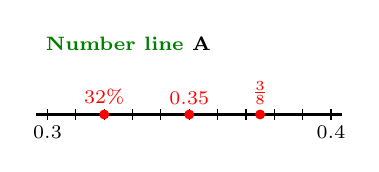
\begin{tikzpicture}[every node/.style={font=\scriptsize}]
\begin{scope}[x=0.36cm, shift={(0.4,0)}]
\node[dhead] at (-0.4,0.9) {\ealkey{Number line} A};
\draw[thick] (-0.4,0) -- (10.4,0);
\foreach \v in {0,...,10} \draw (\v,-0.07) -- (\v,0.07);
\node[nlab] at (0,-0.07)  {$0.3$};
\node[nlab] at (10,-0.07) {$0.4$};
\foreach \v/\lab in {2/{$32\%$}, 5/{$0.35$}, 7.5/{$\tfrac38$}} {
  \fill[ans] (\v,0) circle (1.8pt);
  \node[vans, above, inner sep=1.5pt] at (\v,0.07) {\lab};
}
\end{scope}
\end{tikzpicture}

\column{0.64\textwidth}
\vspace{-1.5em}
\footnotesize
\begin{enumerate}\tightlist
\begin{multicols}{2}
  \item \ealpara{Zapisz $\frac38$ jako \ealkeytr{ułamek dziesiętny} i jako \ealkeytr{procent}.}{Write $\frac38$ as a \ealkey{decimal} and as a \ealkey{percentage}.}
        \ashow{$0.375=37.5\%$}
  \columnbreak
  \item \ealpara{Zapisz $32\,000$ w \ealkeytr{notacji naukowej}.}{Write $32\,000$ in \ealkey{standard form}.}
        \ashow{$3.2\times10^4$}
\end{multicols}
  \item \ealpara{Zaznacz $32\%$, $0.35$ i $\frac38$ na \ealkeytr{osi liczbowej} A. Zapisz je w kolejności, używając $<$.}{Mark $32\%$, $0.35$ and $\frac38$ on \ealkey{number line} A. Write them in order, using $<$.}
        \ashow{$32\%<0.35<\tfrac38$}
\end{enumerate}
\end{columns}
\end{frame}

%------------------------------------------------------------------
% STARTER 1 (2 of 3)
%------------------------------------------------------------------
\begin{frame}[t]{Starter 1: \ealkey{Inequality} Symbols (2 of 3)}
\begin{columns}[T,onlytextwidth]

\column{0.36\textwidth}
\vspace{-0.4em}
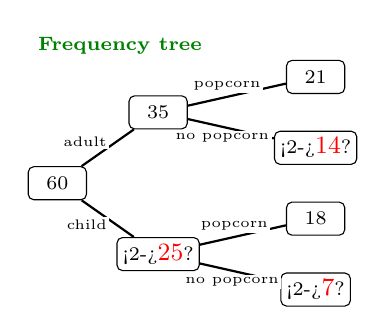
\begin{tikzpicture}[every node/.style={font=\scriptsize}]
\begin{scope}[yshift=-2.55cm]
\node[dhead] at (0,1.75) {\ealkey{Frequency tree}};
\node[ftnode] (t)  at (0.37,0)    {$60$};
\node[ftnode] (a)  at (1.65,0.9)   {$35$};
\node[ftnode] (c)  at (1.65,-0.9)  {\ashowq{25}};
\node[ftnode] (ap) at (3.65,1.35)  {$21$};
\node[ftnode] (an) at (3.65,0.45)  {\ashowq{14}};
\node[ftnode] (cp) at (3.65,-0.45) {$18$};
\node[ftnode] (cn) at (3.65,-1.35) {\ashowq{7}};
\draw[ftarrow] (t) -- node[ftlab, above left=-1pt] {adult} (a);
\draw[ftarrow] (t) -- node[ftlab, below left=-1pt] {child} (c);
\draw[ftarrow] (a) -- node[ftlab, above=1pt, pos=0.4] {popcorn} (ap);
\draw[ftarrow] (a) -- node[ftlab, below=1pt, pos=0.4] {no popcorn} (an);
\draw[ftarrow] (c) -- node[ftlab, above=1pt, pos=0.4] {popcorn} (cp);
\draw[ftarrow] (c) -- node[ftlab, below=1pt, pos=0.4] {no popcorn} (cn);
\end{scope}
\end{tikzpicture}

\column{0.64\textwidth}
\vspace{-1.5em}
\footnotesize
\begin{enumerate}\tightlist
  \item \ealpara{Zapisz $<$ lub $>$.\\[1pt] $3.2\times10^4$ \ablank{$>$} $9.8\times10^3$\\[1pt] $6\times10^{-3}$ \ablank{$<$} $2\times10^{-2}$}{Write $<$ or $>$.\\[1pt] $3.2\times10^4$ \ablank{$>$} $9.8\times10^3$\\[1pt] $6\times10^{-3}$ \ablank{$<$} $2\times10^{-2}$}
  \item \ealpara{$60$ osób obejrzało film. Uzupełnij \ealkeytr{drzewko częstości}.}{$60$ people watched a film. Complete the \ealkey{frequency tree}.}
  \item \ealpara{Dorosły jest wybierany \ealkeytr{losowo}. Znajdź \ealkeytr{prawdopodobieństwo}, że kupił popcorn, jako \ealkeytr{procent}. Zrób to samo dla dziecka. Zapisz $<$ lub $>$ między nimi.}{An adult is chosen \ealkey{at random}. Find the \ealkey{probability} that they bought popcorn, as a \ealkey{percentage}. Do the same for a child. Write $<$ or $>$ between them.}
        \ashow{\ealpara{$\tfrac{21}{35}=60\%$ i $\tfrac{18}{25}=72\%$, więc $60\%<72\%$}{$\tfrac{21}{35}=60\%$ and $\tfrac{18}{25}=72\%$, so $60\%<72\%$}}
\end{enumerate}
\end{columns}
\end{frame}

%------------------------------------------------------------------
% STARTER 1 (3 of 3)
%------------------------------------------------------------------
\begin{frame}[t]{Starter 1: \ealkey{Inequality} Symbols (3 of 3)}
\begin{columns}[T,onlytextwidth]

\column{0.36\textwidth}
\vspace{-0.4em}
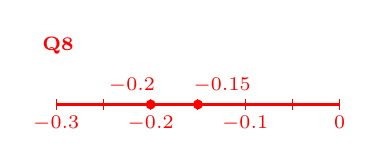
\begin{tikzpicture}[every node/.style={font=\scriptsize}]
\begin{scope}[x=0.12cm, shift={(32.5,0)}, yshift=-5.0cm]
\node[anslab, font=\scriptsize\bfseries, anchor=west] at (-32.5,0.75) {Q8};
\draw[ans] (-30,0) -- (0,0);
\foreach \v in {-30,-25,...,0} \draw[ans, thin] (\v,-0.07) -- (\v,0.07);
\foreach \v/\lab in {-30/-0.3, -20/-0.2, -10/-0.1, 0/0}
  \node[vans, below, inner sep=2pt] at (\v,-0.07) {$\lab$};
\fill[ans] (-20,0) circle (1.8pt);
\fill[ans] (-15,0) circle (1.8pt);
\node[vans, anchor=south east, inner sep=1pt] at (-19.2,0.1) {$-0.2$};
\node[vans, anchor=south west, inner sep=1pt] at (-15.8,0.1) {$-0.15$};
\end{scope}
\end{tikzpicture}

\column{0.64\textwidth}
\vspace{-1.5em}
\footnotesize
\begin{enumerate}\tightlist
  \item \ealpara{$x>0.3$ oznacza ``$x$ jest większe niż $0.3$''. Które z tych może być $x$?\\[1pt] \hspace*{1em}$\tfrac25$ \quad $0.29$ \quad $3\times10^{-1}$ \quad $31\%$ \quad $\tfrac14$\\}{$x>0.3$ means ``$x$ is greater than $0.3$''. Which of these could $x$ be?\\[1pt] \hspace*{1em}$\tfrac25$ \quad $0.29$ \quad $3\times10^{-1}$ \quad $31\%$ \quad $\tfrac14$\\}
        \ashow{\ealpara{$\tfrac25$ i $31\%$, \; ale nie $3\times10^{-1}=0.3$}{$\tfrac25$ and $31\%$, \; but not $3\times10^{-1}=0.3$}}
  \item \ealpara{(Wyzwanie) $0.2>0.15$. Czy $-0.2>-0.15$? Wyjaśnij, używając \ealkeytr{osi liczbowej}.}{(Challenge) $0.2>0.15$. Is $-0.2>-0.15$? Explain using a \ealkey{number line}.}
        \ashow{\ealpara{Nie: \; $-0.2<-0.15$}{No: \; $-0.2<-0.15$}}
\end{enumerate}
\end{columns}
\end{frame}

%------------------------------------------------------------------
% STARTER 2 (1 of 3)
%------------------------------------------------------------------
\begin{frame}[t]{Starter 2: \ealkey{Inequalities} on a \ealkey{Number line} (1 of 3)}
\begin{columns}[T,onlytextwidth]

\column{0.36\textwidth}
\vspace{-0.4em}
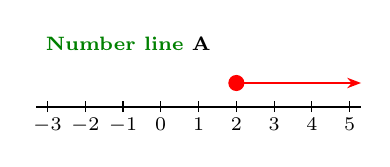
\begin{tikzpicture}[every node/.style={font=\scriptsize}]
\begin{scope}[x=0.48cm, shift={(3.3,0)}]
\node[dhead] at (-3.3,0.8) {\ealkey{Number line} A};
\intline{-3}{5}
\node[ans, closeddot] (a) at (2,\dotheight) {};
\draw[ans, ineq] (a) -- (5.3,\dotheight);
\end{scope}
\end{tikzpicture}

\column{0.64\textwidth}
\vspace{-1.5em}
\footnotesize
\begin{enumerate}\tightlist
\begin{multicols}{2}
  \item \ealpara{Zapisz $0.45$ jako \ealkeytr{ułamek} i jako \ealkeytr{procent}.}{Write $0.45$ as a \ealkey{fraction} and as a \ealkey{percentage}.}
        \ashow{$\tfrac{9}{20}=45\%$}
  \columnbreak
  \item \ealpara{Zapisz $6.1\times10^{-3}$ jako \ealkeytr{liczbę w zwykłej postaci}.}{Write $6.1\times10^{-3}$ as an \ealkey{ordinary number}.}
        \ashow{$0.0061$}
\end{multicols}
  \item \ealpara{Narysuj $x\geq2$ na \ealkeytr{osi liczbowej} A. Czy $x$ może być równe $2$?}{Draw $x\geq2$ on \ealkey{number line} A. Can $x$ be equal to $2$?}
        \ashow{\ealpara{Tak: $\geq$ obejmuje $2$, więc kółko jest wypełnione.}{Yes: $\geq$ includes $2$, so the circle is filled.}}
\end{enumerate}
\end{columns}
\end{frame}

%------------------------------------------------------------------
% STARTER 2 (2 of 3)
%------------------------------------------------------------------
\begin{frame}[t]{Starter 2: \ealkey{Inequalities} on a \ealkey{Number line} (2 of 3)}
\begin{columns}[T,onlytextwidth]

\column{0.36\textwidth}
\vspace{-0.4em}
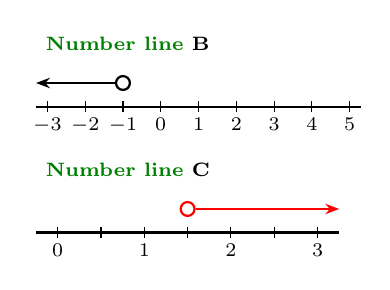
\begin{tikzpicture}[every node/.style={font=\scriptsize}]
\begin{scope}[x=0.48cm, shift={(3.3,0)}, yshift=-1.6cm]
\node[dhead] at (-3.3,0.8) {\ealkey{Number line} B};
\intline{-3}{5}
\node[opendot] (b) at (-1,\dotheight) {};
\draw[ineq] (b) -- (-3.3,\dotheight);
\end{scope}
\begin{scope}[x=1.1cm, shift={(0.25,0)}, yshift=-3.2cm]
\node[dhead] at (-0.25,0.8) {\ealkey{Number line} C};
\draw[thick] (-0.25,0) -- (3.25,0);
\foreach \v in {0,0.5,...,3} \draw (\v,-0.07) -- (\v,0.07);
\foreach \v in {0,...,3} \node[nlab] at (\v,-0.07) {$\v$};
\node[ans, opendot] (c) at (1.5,\dotheight) {};
\draw[ans, ineq] (c) -- (3.25,\dotheight);
\end{scope}
\end{tikzpicture}

\column{0.64\textwidth}
\vspace{-1.5em}
\footnotesize
\begin{enumerate}\tightlist
  \item \ealpara{Zapisz \ealkeytr{nierówność} na \ealkeytr{osi liczbowej} B i dwie \ealkeytr{liczby całkowite}, które ją \ealkeytr{spełniają}.}{Write the \ealkey{inequality} on \ealkey{number line} B, and two \ealkey{integers} that \ealkey{satisfy} it.}
        \ashow{\ealpara{$x<-1$; \; na przykład $-2$ i $-3$}{$x<-1$; \; for example $-2$ and $-3$}}
  \item \ealpara{Narysuj $y>\frac32$ na \ealkeytr{osi liczbowej} C. Czy $y=150\%$ \ealkeytr{spełnia} to?}{Draw $y>\frac32$ on \ealkey{number line} C. Does $y=150\%$ \ealkey{satisfy} it?}
        \ashow{\ealpara{Nie: $150\%=\tfrac32$, nie więcej niż $\tfrac32$.}{No: $150\%=\tfrac32$, not more than $\tfrac32$.}}
  \item \ealpara{Które z tych \ealkeytr{spełniają} $n>4\times10^3$?\\[1pt] \hspace*{1em}$4000$ \quad $3.9\times10^4$ \quad $0.5\times10^4$ \quad $4.01\times10^3$\\}{Which of these \ealkey{satisfy} $n>4\times10^3$?\\[1pt] \hspace*{1em}$4000$ \quad $3.9\times10^4$ \quad $0.5\times10^4$ \quad $4.01\times10^3$\\}
        \ashow{\ealpara{Wszystkie oprócz $4000$, które równa się $4\times10^3$}{All except $4000$, which equals $4\times10^3$}}
\end{enumerate}
\end{columns}
\end{frame}

%------------------------------------------------------------------
% STARTER 2 (3 of 3)
%------------------------------------------------------------------
\begin{frame}[t]{Starter 2: \ealkey{Inequalities} on a \ealkey{Number line} (3 of 3)}
\vspace{-1.5em}
\footnotesize
\begin{enumerate}\tightlist
  \item \ealpara{Mecz kończy się wygraną, remisem lub przegraną. $P(\text{win})=0.35$ i $P(\text{draw})=\frac15$. Znajdź $P(\text{loss})$ jako \ealkeytr{procent}. Zapisz $<$ lub $>$ między $P(\text{win})$ i $P(\text{loss})$.}{A match ends in a win, a draw or a loss. $P(\text{win})=0.35$ and $P(\text{draw})=\frac15$. Find $P(\text{loss})$ as a \ealkey{percentage}. Write $<$ or $>$ between $P(\text{win})$ and $P(\text{loss})$.}
        \ashow{\ealpara{$45\%$, więc $P(\text{win})<P(\text{loss})$}{$45\%$, so $P(\text{win})<P(\text{loss})$}}
  \item \ealpara{(Wyzwanie) $x$ jest \ealkeytr{liczbą całkowitą}, $x>-3$ i $x\leq2$. Wypisz wartości, które może przyjąć $x$.}{(Challenge) $x$ is an \ealkey{integer}, $x>-3$ and $x\leq2$. List the values $x$ can take.}
        \ashow{$-2,\ -1,\ 0,\ 1,\ 2$}
\end{enumerate}
\end{frame}

%------------------------------------------------------------------
% STARTER 3 (1 of 3)
%------------------------------------------------------------------
\begin{frame}[t]{Starter 3: \ealkey{Double Inequalities} (1 of 3)}
\begin{columns}[T,onlytextwidth]

\column{0.36\textwidth}
\vspace{-0.4em}
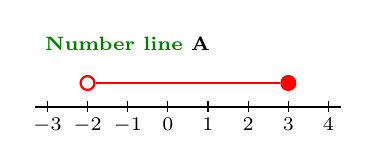
\begin{tikzpicture}[every node/.style={font=\scriptsize}]
\begin{scope}[x=0.51cm, shift={(3.3,0)}]
\node[dhead] at (-3.3,0.8) {\ealkey{Number line} A};
\intline{-3}{4}
\node[ans, opendot]   (l) at (-2,\dotheight) {};
\node[ans, closeddot] (r) at (3,\dotheight)  {};
\draw[ans] (l) -- (r);
\end{scope}
\end{tikzpicture}

\column{0.64\textwidth}
\vspace{-1.5em}
\footnotesize
\begin{enumerate}\tightlist
\begin{multicols}{2}
  \item \ealpara{Zapisz $\frac{7}{20}$ jako \ealkeytr{ułamek dziesiętny} i jako \ealkeytr{procent}.}{Write $\frac{7}{20}$ as a \ealkey{decimal} and as a \ealkey{percentage}.}
        \ashow{$0.35=35\%$}
  \columnbreak
  \item \ealpara{Oblicz $(3\times10^4)\times(2\times10^3)$.}{Work out $(3\times10^4)\times(2\times10^3)$.}
        \ashow{$6\times10^7$}
\end{multicols}
  \item \ealpara{Narysuj $-2<x\leq3$ na \ealkeytr{osi liczbowej} A. Wypisz \ealkeytr{liczby całkowite}, które ją \ealkeytr{spełniają}.}{Draw $-2<x\leq3$ on \ealkey{number line} A. List the \ealkey{integers} that \ealkey{satisfy} it.}
        \ashow{$-1,\ 0,\ 1,\ 2,\ 3$}
\end{enumerate}
\end{columns}
\end{frame}

%------------------------------------------------------------------
% STARTER 3 (2 of 3)
%------------------------------------------------------------------
\begin{frame}[t]{Starter 3: \ealkey{Double Inequalities} (2 of 3)}
\begin{columns}[T,onlytextwidth]

\column{0.36\textwidth}
\vspace{-0.4em}
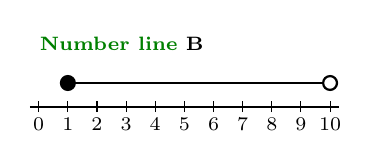
\begin{tikzpicture}[every node/.style={font=\scriptsize}]
\begin{scope}[x=0.37cm, shift={(0.3,0)}, yshift=-1.6cm]
\node[dhead] at (-0.3,0.8) {\ealkey{Number line} B};
\intline{0}{10}
\node[closeddot] (l) at (1,\dotheight)  {};
\node[opendot]   (r) at (10,\dotheight) {};
\draw[thick] (l) -- (r);
\end{scope}
\end{tikzpicture}

\column{0.64\textwidth}
\vspace{-1.5em}
\footnotesize
\begin{enumerate}\tightlist
  \item \ealpara{\ealkeytr{Notacja naukowa} to $A\times10^n$. \ealkeytr{Oś liczbowa} B pokazuje wartości, które może przyjmować $A$. Zapisz je jako \ealkeytr{nierówność podwójną}.}{\ealkey{Standard form} is $A\times10^n$. \ealkey{Number line} B shows the values $A$ can take. Write them as a \ealkey{double inequality}.}
        \ashow{$1\leq A<10$}
  \item \ealpara{Które z tych są w \ealkeytr{notacji naukowej}?\\[1pt] \hspace*{1em}$0.8\times10^3$ \quad $10\times10^2$ \quad $1\times10^5$ \quad $9.9\times10^{-4}$}{Which of these are in \ealkey{standard form}?\\[1pt] \hspace*{1em}$0.8\times10^3$ \quad $10\times10^2$ \quad $1\times10^5$ \quad $9.9\times10^{-4}$}
        \ashow{\ealpara{$1\times10^5$ i $9.9\times10^{-4}$. \; $0.8$ jest mniejsze niż $1$, a $10$ nie jest mniejsze niż $10$.}{$1\times10^5$ and $9.9\times10^{-4}$. \; $0.8$ is less than $1$, and $10$ is not less than $10$.}}
  \item \ealpara{Zapisz $\frac14<x<40\%$ używając \ealkeytr{ułamków dziesiętnych}. Czy $x=\frac13$ to \ealkeytr{spełnia}?}{Write $\frac14<x<40\%$ using \ealkey{decimals}. Does $x=\frac13$ \ealkey{satisfy} it?}
        \ashow{\ealpara{$0.25<x<0.4$; \; tak, $\tfrac13=0.\dot{3}$}{$0.25<x<0.4$; \; yes, $\tfrac13=0.\dot{3}$}}
\end{enumerate}
\end{columns}
\end{frame}

%------------------------------------------------------------------
% STARTER 3 (3 of 3)
%------------------------------------------------------------------
\begin{frame}[t]{Starter 3: \ealkey{Double Inequalities} (3 of 3)}
\begin{columns}[T,onlytextwidth]

\column{0.36\textwidth}
\vspace{-0.4em}
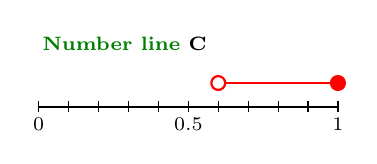
\begin{tikzpicture}[every node/.style={font=\scriptsize}]
\begin{scope}[x=3.8cm, shift={(0.02,0)}, yshift=-3.2cm]
\node[dhead] at (-0.02,0.8) {\ealkey{Number line} C};
\draw[thick] (0,0) -- (1,0);
\foreach \v in {0,0.1,...,1.01} \draw (\v,-0.07) -- (\v,0.07);
\foreach \v/\lab in {0/0, 0.5/0.5, 1/1} \node[nlab] at (\v,-0.07) {$\lab$};
\node[ans, opendot]   (l) at (0.6,\dotheight) {};
\node[ans, closeddot] (r) at (1,\dotheight)   {};
\draw[ans] (l) -- (r);
\end{scope}
\end{tikzpicture}

\column{0.64\textwidth}
\vspace{-1.5em}
\footnotesize
\begin{enumerate}\tightlist
  \item \ealpara{Każde \ealkeytr{prawdopodobieństwo} $p$ \ealkeytr{spełnia} $0\leq p\leq1$. \ealkeytr{Prawdopodobieństwo} deszczu jutro jest większe niż $60\%$. Pokaż wartości, które może przyjmować $p$ na \ealkeytr{osi liczbowej} C, i zapisz je jako \ealkeytr{nierówność podwójną}.}{Every \ealkey{probability} $p$ \ealkey{satisfies} $0\leq p\leq1$. The \ealkey{probability} of rain tomorrow is more than $60\%$. Show the values $p$ can take on \ealkey{number line} C, and write them as a \ealkey{double inequality}.}
        \ashow{$0.6<p\leq1$}
  \item \ealpara{(Wyzwanie) $0.6<P(\text{rain})\leq1$. Zapisz \ealkeytr{nierówność podwójną} dla $P(\text{no rain})$.}{(Challenge) $0.6<P(\text{rain})\leq1$. Write a \ealkey{double inequality} for $P(\text{no rain})$.}
        \ashow{$0\leq P(\text{no rain})<0.4$}
\end{enumerate}
\end{columns}
\end{frame}

%------------------------------------------------------------------
% STARTER 4 (1 of 3)
%------------------------------------------------------------------
\begin{frame}[t]{Starter 4: \ealkey{Solving} \ealkey{Inequalities} (1 of 3)}
\begin{columns}[T,onlytextwidth]

\column{0.36\textwidth}
\vspace{-0.4em}
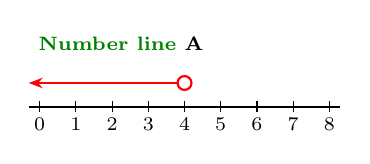
\begin{tikzpicture}[every node/.style={font=\scriptsize}]
\begin{scope}[x=0.46cm, shift={(0.3,0)}]
\node[dhead] at (-0.3,0.8) {\ealkey{Number line} A};
\intline{0}{8}
\node[ans, opendot] (a) at (4,\dotheight) {};
\draw[ans, ineq] (a) -- (-0.3,\dotheight);
\end{scope}
\end{tikzpicture}

\column{0.64\textwidth}
\vspace{-1.5em}
\footnotesize
\begin{enumerate}\tightlist
\begin{multicols}{2}
  \item \ealpara{Zapisz $12\%$ jako \ealkeytr{ułamek dziesiętny} i jako \ealkeytr{ułamek} w \ealkeytr{najprostszej postaci}.}{Write $12\%$ as a \ealkey{decimal} and as a \ealkey{fraction} in its \ealkey{simplest form}.}
        \ashow{$0.12=\tfrac{3}{25}$}
  \columnbreak
  \item \ealpara{Oblicz $(8\times10^6)\div(2\times10^2)$.}{Work out $(8\times10^6)\div(2\times10^2)$.}
        \ashow{$4\times10^4$}
\end{multicols}
  \item \ealpara{\ealkeytr{Rozwiąż} $11>2x+3$. Pokaż rozwiązanie na \ealkeytr{osi liczbowej} A.}{\ealkey{Solve} $11>2x+3$. Show the solution on \ealkey{number line} A.}
        \ashow{\ealpara{$8>2x$, więc $4>x$, co daje $x<4$}{$8>2x$, so $4>x$, which is $x<4$}}
\end{enumerate}
\end{columns}
\end{frame}

%------------------------------------------------------------------
% STARTER 4 (2 of 3)
%------------------------------------------------------------------
\begin{frame}[t]{Starter 4: \ealkey{Solving} \ealkey{Inequalities} (2 of 3)}
\vspace{-1.5em}
\footnotesize
\begin{enumerate}\tightlist
  \item \ealpara{$30\%$ z $y$ jest mniejsze niż $6$. Zapisz \ealkeytr{nierówność} i ją \ealkeytr{rozwiąż}.}{$30\%$ of $y$ is less than $6$. Write an \ealkey{inequality} and \ealkey{solve} it.}
        \ashow{\ealpara{$0.3y<6$, więc $y<20$}{$0.3y<6$, so $y<20$}}
  \item \ealpara{\ealkeytr{Rozwiąż} $3m\leq1.2\times10^5$, podając $m$ w \ealkeytr{notacji naukowej}.}{\ealkey{Solve} $3m\leq1.2\times10^5$, giving $m$ in \ealkey{standard form}.}
        \ashow{$m\leq4\times10^4$}
\end{enumerate}
\end{frame}

%------------------------------------------------------------------
% STARTER 4 (3 of 3)
%------------------------------------------------------------------
\begin{frame}[t]{Starter 4: \ealkey{Solving} \ealkey{Inequalities} (3 of 3)}
\begin{columns}[T,onlytextwidth]

\column{0.36\textwidth}
\vspace{-0.4em}
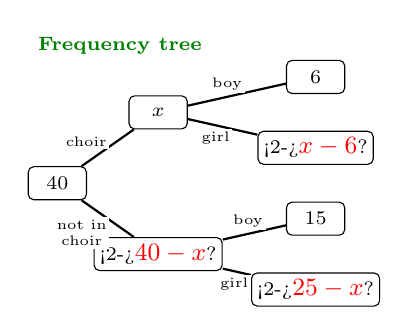
\begin{tikzpicture}[every node/.style={font=\scriptsize}]
\begin{scope}[yshift=-2.65cm]
\node[dhead] at (0,1.75) {\ealkey{Frequency tree}};
\node[ftnode] (t)  at (0.37,0)    {$40$};
\node[ftnode] (c)  at (1.65,0.9)   {$x$};
\node[ftnode] (n)  at (1.65,-0.9)  {\ashowq{$40-x$}};
\node[ftnode] (cb) at (3.65,1.35)  {$6$};
\node[ftnode] (cg) at (3.65,0.45)  {\ashowq{$x-6$}};
\node[ftnode] (nb) at (3.65,-0.45) {$15$};
\node[ftnode] (ng) at (3.65,-1.35) {\ashowq{$25-x$}};
\draw[ftarrow] (t) -- node[ftlab, above left=-1pt] {choir} (c);
\draw[ftarrow] (t) -- node[ftlab, below left=-1pt, align=center] {not in\\choir} (n);
\draw[ftarrow] (c) -- node[ftlab, above=1pt, pos=0.4] {boy} (cb);
\draw[ftarrow] (c) -- node[ftlab, below=1pt, pos=0.4] {girl} (cg);
\draw[ftarrow] (n) -- node[ftlab, above=1pt, pos=0.4] {boy} (nb);
\draw[ftarrow] (n) -- node[ftlab, below=1pt, pos=0.4] {girl} (ng);
\end{scope}
\end{tikzpicture}

\column{0.64\textwidth}
\vspace{-1.5em}
\footnotesize
\begin{enumerate}\tightlist
  \item \ealpara{$40$ uczniów zostało zapytanych, czy śpiewają w chórze. Uzupełnij \ealkeytr{drzewko częstości} używając $x$.}{$40$ pupils were asked if they sing in the choir. Complete the \ealkey{frequency tree} in terms of $x$.}
  \item \ealpara{W chórze jest więcej dziewcząt niż chłopców. Zapisz \ealkeytr{nierówność} z $x$ i ją \ealkeytr{rozwiąż}.}{There are more girls than boys in the choir. Write an \ealkey{inequality} in $x$ and \ealkey{solve} it.}
        \ashow{\ealpara{$x-6>6$, więc $x>12$}{$x-6>6$, so $x>12$}}
  \item \ealpara{(Wyzwanie) \ealkeytr{Prawdopodobieństwo}, że losowo wybrany uczeń jest w chórze, jest również mniejsze niż $0.4$. Wypisz wartości, które może przyjmować $x$.}{(Challenge) The \ealkey{probability} that a pupil chosen \ealkey{at random} is in the choir is also less than $0.4$. List the values $x$ can take.}
        \ashow{\ealpara{$0.4\times40=16$, więc $12<x<16$: \; $x=13$, $14$ lub $15$}{$0.4\times40=16$, so $12<x<16$: \; $x=13$, $14$ or $15$}}
\end{enumerate}
\end{columns}
\end{frame}

%------------------------------------------------------------------
% STARTER 5 (1 of 3)
%------------------------------------------------------------------
\begin{frame}[t]{Starter 5: \ealkey{Solving} \ealkey{Double Inequalities} (1 of 3)}
\vspace{-1.5em}
\footnotesize
\begin{enumerate}\tightlist
  \item \ealpara{Zapisz $\frac18$ jako \ealkeytr{ułamek dziesiętny} i jako \ealkeytr{procent}.}{Write $\frac18$ as a \ealkey{decimal} and as a \ealkey{percentage}.}
        \ashow{$0.125=12.5\%$}
  \item \ealpara{Zapisz $0.0032$ w \ealkeytr{notacji naukowej}.}{Write $0.0032$ in \ealkey{standard form}.}
        \ashow{$3.2\times10^{-3}$}
  \item \ealpara{\ealkeytr{Rozwiąż} $5x-3\leq2x+9$.}{\ealkey{Solve} $5x-3\leq2x+9$.}
        \ashow{\ealpara{$3x\leq12$, więc $x\leq4$}{$3x\leq12$, so $x\leq4$}}
\end{enumerate}
\end{frame}

%------------------------------------------------------------------
% STARTER 5 (2 of 3)
%------------------------------------------------------------------
\begin{frame}[t]{Starter 5: \ealkey{Solving} \ealkey{Double Inequalities} (2 of 3)}
\begin{columns}[T,onlytextwidth]

\column{0.36\textwidth}
\vspace{-0.4em}
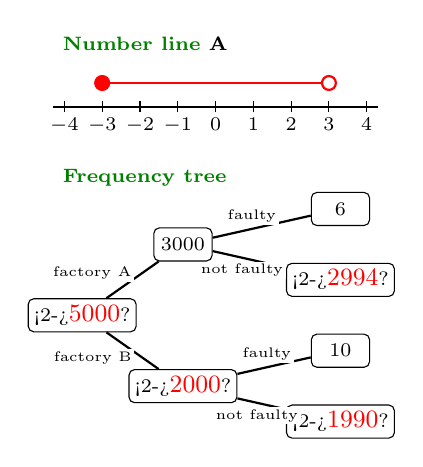
\begin{tikzpicture}[every node/.style={font=\scriptsize}]
\begin{scope}[x=0.48cm, shift={(4.3,0)}]
\node[dhead] at (-4.3,0.8) {\ealkey{Number line} A};
\intline{-4}{4}
\node[ans, closeddot] (l) at (-3,\dotheight) {};
\node[ans, opendot]   (r) at (3,\dotheight)  {};
\draw[ans] (l) -- (r);
\end{scope}
\begin{scope}[yshift=-2.65cm]
\node[dhead] at (0,1.75) {\ealkey{Frequency tree}};
\node[ftnode] (t)  at (0.37,0)    {\ashowq{5000}};
\node[ftnode] (a)  at (1.65,0.9)   {$3000$};
\node[ftnode] (b)  at (1.65,-0.9)  {\ashowq{2000}};
\node[ftnode] (af) at (3.65,1.35)  {$6$};
\node[ftnode] (an) at (3.65,0.45)  {\ashowq{2994}};
\node[ftnode] (bf) at (3.65,-0.45) {$10$};
\node[ftnode] (bn) at (3.65,-1.35) {\ashowq{1990}};
\draw[ftarrow] (t) -- node[ftlab, above left=-1pt] {factory A} (a);
\draw[ftarrow] (t) -- node[ftlab, below left=-1pt] {factory B} (b);
\draw[ftarrow] (a) -- node[ftlab, above=1pt, pos=0.4] {faulty} (af);
\draw[ftarrow] (a) -- node[ftlab, below=1pt, pos=0.4] {not faulty} (an);
\draw[ftarrow] (b) -- node[ftlab, above=1pt, pos=0.4] {faulty} (bf);
\draw[ftarrow] (b) -- node[ftlab, below=1pt, pos=0.4] {not faulty} (bn);
\end{scope}
\end{tikzpicture}

\column{0.64\textwidth}
\vspace{-1.5em}
\footnotesize
\begin{enumerate}\tightlist
\begin{multicols}{2}
  \item \ealpara{Firma wyprodukowała $5\times10^3$ telefonów. Uzupełnij \ealkeytr{drzewko częstości}.}{A company made $5\times10^3$ phones. Complete the \ealkey{frequency tree}.}
  \columnbreak
  \item \ealpara{Zapisz \ealkeytr{prawdopodobieństwo}, że telefon z fabryki A jest wadliwy, w \ealkeytr{notacji naukowej}. Zrób to samo dla fabryki B. Zapisz $<$ lub $>$ między nimi.}{Write the \ealkey{probability} that a phone from factory A is faulty in \ealkey{standard form}. Do the same for factory B. Write $<$ or $>$ between them.}
        \ashow{$\tfrac{6}{3000}=2\times10^{-3}\ <\ \tfrac{10}{2000}=5\times10^{-3}$}
\end{multicols}
  \item \ealpara{\ealkeytr{Rozwiąż} $-5\leq2x+1<7$. Pokaż to na \ealkeytr{osi liczbowej} A i wypisz \ealkeytr{liczby całkowite}, które ją \ealkeytr{spełniają}.}{\ealkey{Solve} $-5\leq2x+1<7$. Show it on \ealkey{number line} A, and list the \ealkey{integers} that \ealkey{satisfy} it.}
        \ashow{$-3\leq x<3$; \; $-3,\ -2,\ -1,\ 0,\ 1,\ 2$}
\end{enumerate}
\end{columns}
\end{frame}

%------------------------------------------------------------------
% STARTER 5 (3 of 3)
%------------------------------------------------------------------
\begin{frame}[t]{Starter 5: \ealkey{Solving} \ealkey{Double Inequalities} (3 of 3)}
\vspace{-1.5em}
\footnotesize
\begin{enumerate}\tightlist
  \item \ealpara{\ealkeytr{Obciążony} spinner zatrzymuje się na czerwonym z \ealkeytr{prawdopodobieństwem} $2x-0.4$. Użyj $0\leq P(\text{red})\leq1$, aby znaleźć wartości, które może przyjmować $x$.}{A \ealkey{biased} spinner lands on red with \ealkey{probability} $2x-0.4$. Use $0\leq P(\text{red})\leq1$ to find the values $x$ can take.}
        \ashow{\ealpara{$0.4\leq2x\leq1.4$, więc $0.2\leq x\leq0.7$}{$0.4\leq2x\leq1.4$, so $0.2\leq x\leq0.7$}}
  \item \ealpara{(Wyzwanie) Worek zawiera $4$ czerwone i $n$ niebieskich liczników. $P(\text{red})<20\%$. Znajdź najmniejszą wartość, jaką może przyjąć $n$.}{(Challenge) A bag holds $4$ red and $n$ blue counters. $P(\text{red})<20\%$. Find the smallest value $n$ can take.}
        \ashow{\ealpara{$0.2(4+n)>4$, więc $4+n>20$ i $n>16$; \; $n=17$}{$0.2(4+n)>4$, so $4+n>20$ and $n>16$; \; $n=17$}}
\end{enumerate}
\end{frame}

\end{document}